\documentclass[11pt,a4paper]{article}
\usepackage[margin=22mm]{geometry}
\usepackage[T1]{fontenc}
\usepackage{lmodern,amsmath,amssymb,booktabs,array,graphicx,tikz,listings,xcolor,hyperref}
\usetikzlibrary{arrows.meta,positioning,shapes.geometric,calc}
\hypersetup{pdftitle={Cedar-8f2c student reference},pdfauthor={Cedar-8f2c},colorlinks=true,linkcolor=blue,urlcolor=blue}
\lstset{basicstyle=\ttfamily\small,breaklines=true,columns=fullflexible,frame=single}
\newcommand{\bits}[1]{\texttt{#1}}
\newcommand{\reference}{\noindent\textbf{Student reference.} This is an anonymous, editable reconstruction of the supplied student report. It preserves the student's approach and reported results. Editorial verification notes and assignment clarifications are labeled separately. It is not a newly corrected solution or a claim of full fault coverage. The accompanying anonymized PDF preserves the original evidence.\par}
\title{Homework 2: Signature analysis\\Student reference}
\author{Cedar-8f2c}
\date{}
\begin{document}
\maketitle
\reference

\section{Assignment clarification}
The first question uses a modular signature analyzer with characteristic polynomial $c(x)=1+x+x^4$.
The supplementary announcement says that the printed table's $F$ column contains errors. The four input columns $X_1,\ldots,X_4$ remain usable. Each input vector must pass through the circuit under test (CUT), and the resulting $F$ sequence must enter the LFSR. The report should compare the simulated signature with polynomial division. Parts (a) and (b) may use separate simulations, but both waveforms and explanations are required.

\section{Part 1: Four-bit signature analyzer}
The student's reconstructed modular LFSR has four state bits $q_0,\ldots,q_3$. With input bit $m$, its implemented recurrence is
\begin{align*}
q_0^+&=m\oplus q_3,\\
q_1^+&=q_0\oplus q_3,\\
q_2^+&=q_1,\\
q_3^+&=q_2.
\end{align*}
Reset initializes all four state bits to zero. The enable signal controls state updates.
\begin{figure}[ht]\centering
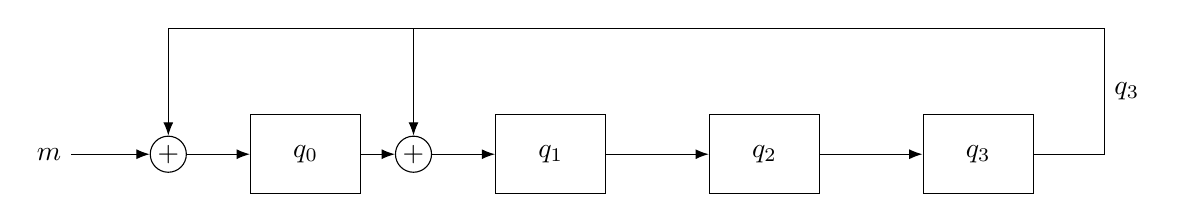
\begin{tikzpicture}[>=Latex,b/.style={draw,minimum width=14mm,minimum height=10mm}]
\node[b] (d0) {$q_0$};
\node[b,right=17mm of d0] (d1) {$q_1$};
\node[b,right=13mm of d1] (d2) {$q_2$};
\node[b,right=13mm of d2] (d3) {$q_3$};
\node[draw,circle,left=8mm of d0,inner sep=1pt] (x0) {$+$};
\node[draw,circle,left=8mm of d1,inner sep=1pt] (x1) {$+$};
\draw[->] (x0)--(d0);\draw[->](d0)--(x1);\draw[->](x1)--(d1);
\draw[->](d1)--(d2);\draw[->](d2)--(d3);
\draw[<-](x0.west)--++(-10mm,0)node[left] {$m$};
\draw (d3.east)--++(9mm,0)coordinate(out);
\draw[->](out)--node[right] {$q_3$}++(0,16mm)-|(x0.north);
\draw[->] ($(x1)+(0,16mm)$)--(x1.north);
\end{tikzpicture}
\caption{Editable reconstruction of the modular LFSR. A circle marked $+$ denotes XOR.}
\end{figure}

\subsection{Reported good-circuit signature}
The report states that the 15 CUT input patterns produce a final good-circuit signature of \bits{1100}. With bit three representing $x^3$, this is $x^3+x^2$. It writes
\[
m(x)=x^{10}+x^6+x^2+x+1
\]
and the division
\[
m(x)=(x^4+x+1)(x^6+x^3+1)+(x^3+x^2)
\qquad\text{over }GF(2).
\]
The original writes a minus before $x^3$ in the quotient. In $GF(2)$ the plus and minus signs are identical. The reconstruction uses plus to make the field arithmetic explicit.

\subsection{Reported line-a stuck-at-zero signature}
For line $a$ stuck at zero, the source report gives \bits{0101}, equivalent to $x^2+1$. Its polynomial argument is
\[
m_a(x)=x^2+1=(x^4+x+1)\cdot0+(x^2+1).
\]
The accompanying original waveforms label these final values. These are retained as reported results, and the original Verilog is published independently so its actual timing and CUT equations can be checked.

\paragraph{Editorial verification notes.}
Input ordering, the reset interval, and exactly which enabled edges consume the 15 patterns all affect the signature.
In the retained testbench, pattern 1 is present during reset, the design becomes enabled with pattern 2, and pattern 15 remains for an extra enabled edge. The published simulation must therefore be interpreted with those details.
The CUT source also repeats one product term. A report's arithmetic agreement does not by itself prove that the implemented CUT matches every gate in the assignment drawing.

\section{Part 2: Syndrome compaction}
The original circuit takes the eight input positions from
\[
\begin{split}
a&=\bits{11110000},\qquad b=\bits{11001100},\\
c&=\bits{10101010},\qquad d=\bits{10101110}.
\end{split}
\]
Its logic is $e=ab$, $f=\overline{cd}$, and $z=\overline{e+f}$. In the good circuit,
\[
e=\bits{11000000},\quad f=\bits{01010101},\quad z=\bits{00101010}.
\]
\begin{figure}[ht]\centering
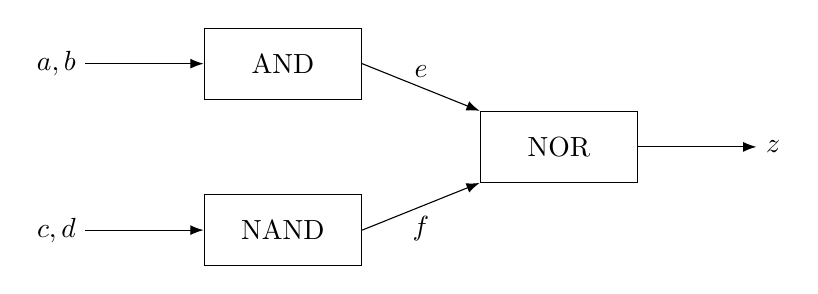
\begin{tikzpicture}[>=Latex,b/.style={draw,minimum width=20mm,minimum height=9mm}]
\node[b] (and) {AND};
\node[b,below=12mm of and] (nand) {NAND};
\node[b,right=25mm of $(and)!.5!(nand)$] (nor) {NOR};
\draw[<-](and.west)--++(-15mm,0)node[left] {$a,b$};
\draw[<-](nand.west)--++(-15mm,0)node[left] {$c,d$};
\draw[->](and.east)--node[above] {$e$}(nor.north west);
\draw[->](nand.east)--node[below] {$f$}(nor.south west);
\draw[->](nor.east)--++(15mm,0)node[right] {$z$};
\end{tikzpicture}
\caption{Logic used for the student's syndrome-compaction calculation.}
\end{figure}
The student collapses faults to the representative list
\[
\{a/0,\ a/1,\ b/1,\ c/0,\ c/1,\ d/1\}.
\]
The report's complete response and compaction table is reproduced below.
\begin{center}\small
\begin{tabular}{lccc}
\toprule
Fault & Response $z$ & Parity & One's count\\\midrule
No fault & 0010\,1010 & Odd & 3\\
$a/0$ & 1010\,1010 & Even & 4\\
$a/1$ & 0010\,0010 & Even & 2\\
$b/1$ & 0000\,1010 & Even & 2\\
$c/0$ & 0000\,0000 & Even & 0\\
$c/1$ & 0010\,1110 & Even & 4\\
$d/1$ & 0010\,1010 & Odd & 3\\
\bottomrule
\end{tabular}\end{center}
Only $d/1$ in the listed representatives escapes both compactors. The supplied vectors never apply $(c,d)=(1,0)$. The faulty output therefore equals the good output at every position, so this case lacks fault activation or propagation before compaction. It is not an example of two different response sequences colliding solely because of the compactor.
\paragraph{Editorial verification note.}
This table refers to the listed collapsed representatives. It must not be described as a complete listing of every original circuit-line fault without expanding the equivalence classes and checking them.

\section{Retained source set}
The two top modules \bits{HW2\_1\_a} and \bits{HW2\_1\_b} instantiate shared modules from \bits{Sub\_module.v}. Their separate testbenches remain available. The project-directory copies of these five files match the submitted sources and are omitted as duplicates. The two parts should be elaborated separately by specifying the intended testbench top.
\section{Repository verification}
Icarus Verilog 13.0 compiled and executed both retained testbenches. Observing the final state at 180 ns reproduces the report's good-circuit signature \bits{1100} and faulty-circuit signature \bits{0101}. The compiler warns that \bits{b} in \bits{CUT\_fault} is an implicitly declared wire. The source is retained without changing that declaration. These results verify the reported simulations, while circuit transcription and the wider fault model remain separate questions.
\end{document}
